\section{Liouville equation and the pendulum}

Consider the pendulum of length l and mass m in a gravitational field
g. The kinetic energy and potential energy are
\begin{equation}
    T=\frac{1}{2}ml^2\dot{\theta}^2
\end{equation}
and 
\begin{equation}
    V=mgl(1-\cos\theta)
\end{equation}

\subsection{}
%Derive the Hamiltonian and write down Hamilton’s equations.
Starting from the Lagrangian, 
\begin{equation*}
    \mathcal{L}(\theta,\dot{\theta},t)\equiv T-V = \frac{1}{2}ml^2\dot{\theta}^2 - mgl(1 - \cos\theta),
\end{equation*}
we can find the generalized momentum by
\begin{align*}
    p\equiv\frac{\partial\mathcal{L}}{\partial\dot{q}}=ml^2\dot{\theta}.
\end{align*}
Then the Hamiltonian is
\begin{align*}
    \mathcal{H}&\equiv T+V\\
    \mathcal{H}&=\frac{1}{2}ml^2\dot{\theta}^2+mgl(1-\cos\theta)\\
    \mathcal{H}&=\frac{1}{2}\frac{p^2}{ml^2}+mgl(1-\cos\theta).
\end{align*}

Hamilton's equations are:
\begin{align*}
    \dot{p}&\equiv-\frac{\partial\mathcal{H}}{\partial\theta}=-mgl\sin\theta\\
    \dot{q}&\equiv\frac{\partial\mathcal{H}}{\partial p}=\frac{p}{ml^2}=\dot{\theta}
\end{align*}

\subsection{}
%Transform these equations to a non-dimensional set of variables $(q,p)\to(z_1,z_2)$ such that $\tau=\omega t$ where $\omega^2=g/l$ and the dimensionless energy is:
% \begin{equation}
%     \varepsilon\equiv\frac{E}{mgl}=\frac{1}{2}z_2^2+(1-\cos z_1)
% \end{equation}
% Show that $\tau_0=2\pi/\omega$ is the period of small oscillations  for this system.
From the dimensionless energy $\varepsilon=E/mgl$ 
\begin{align*}
    \varepsilon&=\frac{1}{mgl}\left[\frac{1}{2}ml^2\dot{\theta}^2+mgl(1-\cos\theta)\right]\\
    &=\frac{1}{2}\frac{l}{g}\dot{\theta} + (1-\cos\theta),
\end{align*}
we can find the dimensionless variables as
\begin{align*}
    z_1\equiv\theta\\
    z_2\equiv\frac{l}{g}\dot{\theta}=\frac{\dot{\theta}}{\omega^2}
\end{align*}
where $\omega^2=g/l$.

Knowing that the equation of motion for this system is 
\begin{equation*}
    \Ddot{\theta}=-\frac{g}{l}\sin\theta
    \label{eq:pendEqMotion}
\end{equation*}
we can find that the solution for this differential equation in the small angle approximation will be given by
\begin{equation*}
\frac{dz_2}{d\tau}=\frac{d}{dt}
\frac{\Ddot{\theta}}{\omega^2}=    
\end{equation*}


then, we can show that
$\tau_0=2\pi/\omega$.

\subsection{}
%Sketch the phase portrait in these units, paying special attention to
% the three domains: 1) $\varepsilon<2$, the oscillation  or libration regime; 2) $\varepsilon>2$, the rotation regime 3)$\varepsilon=2$, the critical infinite period, the separatrix.

\begin{figure}
    \centering
    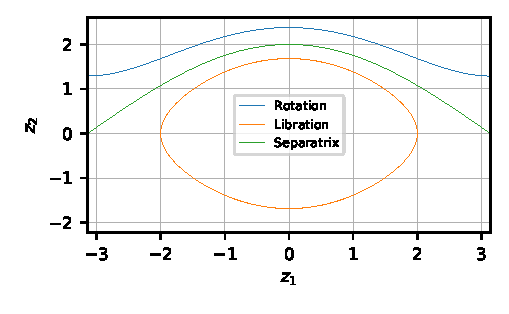
\includegraphics{CodeAndFigures/PendulumPhaseSpace.pdf}
    \caption{Phase Space of a pendulum in rotation ($\varepsilon>2$), libration ($\varepsilon<2$) and separatrix ($\varepsilon=2$).}
    \label{fig:pendPhaseSpace}
\end{figure}

We can integrate the pendulum's equation of motion \ref{eq:pendEqMotion} using a 4th order Runge-Kutta and the initial conditions listed in table \ref{tab:pendulumIV}.

\begin{table}
    \centering
    \begin{tabular}{lrrr}
\toprule
{} &  $z_1$ &  $z_2$ &  Energy \\
\midrule
Rotation   &  -4.71 &   1.91 &    2.83 \\
Libration  &  -1.57 &   0.91 &    1.42 \\
Separatrix &  -4.71 &   1.41 &    2.00 \\
\bottomrule
\end{tabular}

    \caption{Initial conditions used for obtaining the phase-space of the pendulum for rotation, libration and separatrix.}
    \label{tab:pendulumIV}
\end{table}

Figure \ref{fig:pendPhaseSpace} shows the phase space in the three domains: rotation, libration and separatrix.

\subsection{}
Considering a disk-like of initial conditions enclosed within a circle centered at $(q,p)=(z_1,z_2)=(0,1)$ with radius of $1/2$ as shown in Figure \ref{fig:MartinsUs}
\begin{figure}
    \centering
    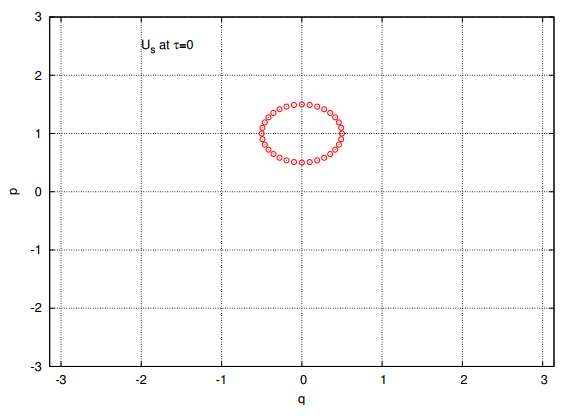
\includegraphics[width=\columnwidth]{CodeAndFigures/Fig1InitialConditionsUs.png}
    %\caption{Caption}
    \label{fig:my_label}
\end{figure}
%Consider a disk-like domain of initial configurations $U_s$ enclosed
% within the circle centered at $(q,p)=(z_1,z_2)=(0,1)$ with radius
% of $1/2$ in these units. See Fig. 1 for a plot of these initial conditions. Compute the evolution of the disk from $\tau=0$ to each of $\tau=0.25\tau_0,0.5\tau_0,\mathrm{and}\tau_0$.
% Remarks:
%     \begin{itemize}
%     \item Argue that it is sufficient to compute the
%           trajectories on the
%           circle at edge of the disk. In other words, a point
%           on the inside of the disk can not pass through
%           a boundary point.
%     \item You may solve this any way you like. E.g. there is 
%           an analytic solution in terms of elliptic 
%           integrals. But I recommend an numerical solution, 
%           using your RK4 routine to solve the equations of
%           motion for say 32 points equally spaced around the 
%           circle at the perimeter of $U_s$ at $\tau = 0$.
%     \item For insight consider this problem in the small 
%           angle limit. In this limit, the solution is 
%           analytic. If you have any worries about your 
%           solution, make sure it agrees with the small angle 
%           limit.
%     \end{itemize}

\begin{figure}[h!]
    \centering
    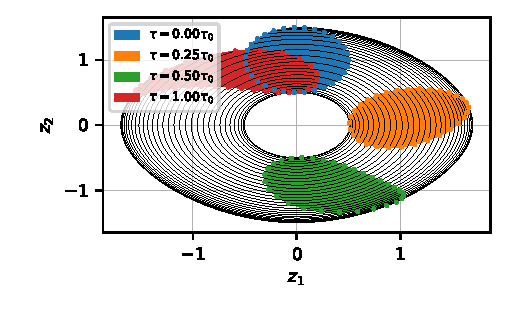
\includegraphics{CodeAndFigures/PendulumPhaseSpaceUs2d.pdf}
    \caption{PhaseSpace using initial conditions }
    \label{fig:pend2d}
\end{figure}

\subsection{}
% \item Repeat the experiment but now with the circle centered at $(q,p)=(0,1.5)$ Note: some points will be on or near the seperatrix. Compute the evolution of the disk for $\tau=0,0.2\tau_0,0.4\tau_0,\mathrm{and}0.75\tau_0$.[NB: the “evolution” at t = 0 is the initial condition, of course.]
\begin{figure}[h!]
    \centering
    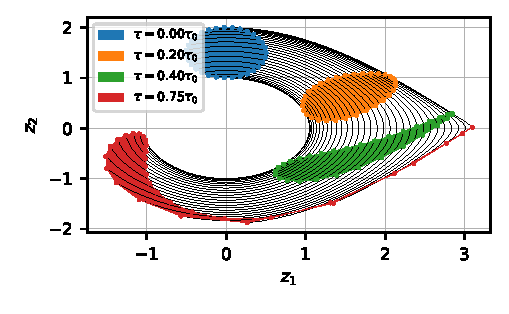
\includegraphics{CodeAndFigures/PendulumPhaseSpaceUs2e.pdf}
    \caption{Caption}
    \label{fig:pend2e}
\end{figure}

\subsection{}
%Repeat the experiment but now with the circle centered at  $(q,p)=(0,2)$. Compute the evolution at times $\tau=0,0.1\tau_0,0.25\tau_0,\mathrm{and}0.5\tau_0$

\begin{figure}[h!]
    \centering
    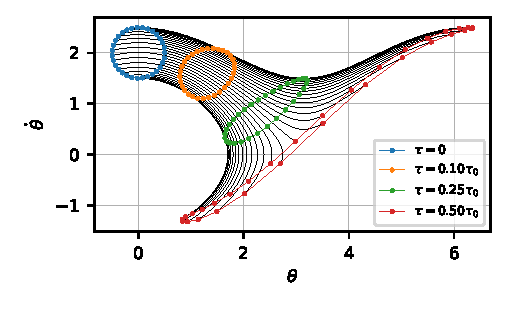
\includegraphics{CodeAndFigures/PendulumPhaseSpaceUs2f.pdf}
    \caption{Caption}
    \label{fig:pend2f}
\end{figure}

\subsection{}
%For each of the three experiment with different disk centers, make
% a plot the disk at each of these times in the $(q,p)$ plane (e.g.
% a phase portrait). Interpret the results. Is Liouville’s theorem obeyed?